\documentclass[border=12pt]{standalone}
\usepackage{tikz}
\usetikzlibrary{arrows.meta, positioning, calc, decorations.pathreplacing}
\usepackage{amsmath}
\usepackage{xcolor}

\definecolor{navy}{HTML}{1E2761}
\definecolor{accent}{HTML}{408EC6}
\definecolor{iceblue}{HTML}{CADCFC}
\definecolor{lightbg}{HTML}{F4F6FB}
\definecolor{muted}{HTML}{6B7280}

\begin{document}
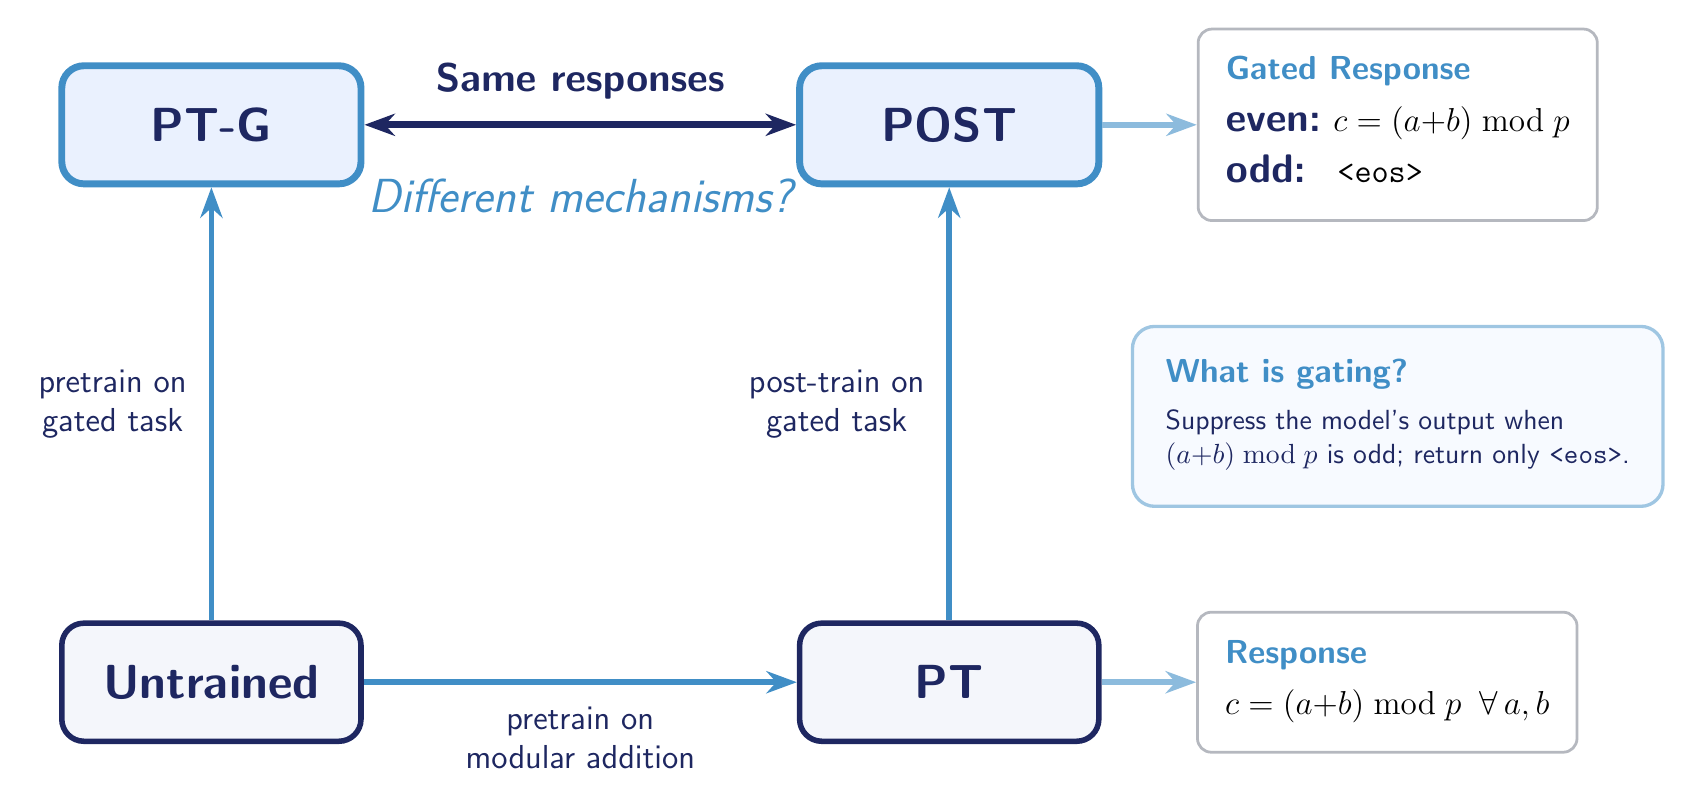
\begin{tikzpicture}[
    node distance=5.5cm and 5.5cm,
    box/.style={
        rectangle, rounded corners=8pt, draw=navy, line width=2pt,
        fill=lightbg, minimum width=3.8cm, minimum height=1.5cm,
        font=\LARGE\bfseries\sffamily, text=navy, align=center
    },
    highlight/.style={
        rectangle, rounded corners=8pt, draw=accent, line width=2.5pt,
        fill=iceblue!40, minimum width=3.8cm, minimum height=1.5cm,
        font=\LARGE\bfseries\sffamily, text=navy, align=center
    },
    arr/.style={-{Stealth[length=11pt, width=8pt]}, line width=2pt, accent},
    darr/.style={{Stealth[length=11pt, width=8pt]}-{Stealth[length=11pt, width=8pt]}, line width=2.5pt, navy},
    lbl/.style={font=\large\sffamily, align=center, text=navy, fill=white, inner sep=4pt, rounded corners=2pt},
    respbox/.style={rectangle, rounded corners=5pt, draw=muted!50, line width=1pt, fill=white, inner sep=10pt},
    callout/.style={rectangle, rounded corners=8pt, draw=accent!50, line width=1.2pt, fill=iceblue!15, inner sep=12pt, font=\normalsize\sffamily, text=navy},
]

% Nodes
\node[box] (untrained) {Untrained};
\node[box, right=of untrained] (pt) {PT};
\node[highlight, above=of untrained] (ptg) {PT-G};
\node[highlight, above=of pt] (post) {POST};

% Bottom arrow: Untrained -> PT
\draw[arr] (untrained) -- node[lbl, below=4pt] {pretrain on\\modular addition} (pt);

% Left arrow: Untrained -> PT-G
\draw[arr] (untrained) -- node[lbl, left=4pt] {pretrain on\\gated task} (ptg);

% Right arrow: PT -> POST
\draw[arr] (pt) -- node[lbl, left=4pt] {post-train on\\gated task} (post);

% Top double arrow: PT-G <-> POST with "Same responses"
\draw[darr] (ptg) -- node[lbl, above=4pt, font=\Large\sffamily\bfseries, text=navy] {Same responses} (post);

% Question below the top arrow
\node[font=\LARGE\itshape\sffamily, text=accent] at ($(ptg)!0.5!(post) + (0,-0.9)$) {Different mechanisms?};

% Response box to the right of POST with "Gated Output" title
\node[respbox, right=1.2cm of post, anchor=west] (gated_resp) {%
    \begin{tabular}{@{}l@{}}
    \textcolor{accent}{\large\textsf{\textbf{Gated Response}}}\\[6pt]
    \textcolor{navy}{\Large\textsf{\textbf{even:}}} {\large $c = (a{+}b) \bmod p$}\\[5pt]
    \textcolor{navy}{\Large\textsf{\textbf{odd:\phantom{n}}}} {\large \texttt{<eos>}}
    \end{tabular}
};
\draw[arr, accent!60] (post.east) -- (gated_resp.west);

% Response box to the right of PT
\node[respbox, right=1.2cm of pt, anchor=west] (pt_resp) {%
    \begin{tabular}{@{}l@{}}
    \textcolor{accent}{\large\textsf{\textbf{Response}}}\\[6pt]
    {\large $c = (a{+}b) \bmod p \;\; \forall \, a, b$}
    \end{tabular}
};
\draw[arr, accent!60] (pt.east) -- (pt_resp.west);

% Callout box: what is gating — vertically centered between response boxes, horizontally centered on them
\coordinate (mid_resp) at ($(gated_resp.south)!0.5!(pt_resp.north)$);
\node[callout, anchor=center] (gating_def) at (mid_resp -| gated_resp.center) {%
    \begin{tabular}{@{}l@{}}
    \textcolor{accent}{\large\textsf{\textbf{What is gating?}}}\\[5pt]
    {\normalsize Suppress the model's output when}\\
    {\normalsize $(a{+}b) \bmod p$ is odd; return only \texttt{<eos>}.}
    \end{tabular}
};

\end{tikzpicture}
\end{document}
